\documentclass[a1paper,fontsize=24.88pt,twoside=false,english,DIV=calc,NET]{scrartcl}

\usepackage{wrapfig}

\usepackage{svg}
% size should not be changed unless explicitely instructed otherwise
\usepackage{geometry}
\geometry{paperwidth=600mm, paperheight=800mm, left=35mm,right=35mm, top=35mm, bottom=35mm} % I8 framesize

% sizes

\newcommand{\headervspace}{26mm} % A1/I8
\newcommand{\logoheight}{26mm} % A1/I8

\usepackage{posterstyle}

% ===============================================================
% Font settings
% ===============================================================
\usepackage{helvet}
\renewcommand{\familydefault}{\sfdefault}
\fontfamily{phv}\selectfont
\renewcommand{\rmdefault}{lhv}
\renewcommand{\seriesdefault}{m}
\renewcommand{\shapedefault}{n}
\DeclareSymbolFont{operators}{OT1}{cmbr}{m}{n}
\DeclareSymbolFont{letters}{OML}{cmbrm}{m}{it}
\DeclareSymbolFont{symbols}{OMS}{cmbrs}{m}{n}
% ===============================================================

% Type and title of your work, please adhere to the following format:
% {Bachelor' Thesis | Master's Thesis | Interdisciplinary Project | Guided Research}: title,
\def\titletext{Bachelor's Thesis: Performance-Analysis of VPP}

% Adapt font size to fit in a single line
\newcommand{\titlefontsize}{\fontsize{36}{40}\selectfont} % A1/I8

% Fill in the name of the persons
\def\presenter{Peter Okelmann}
\def\advisor{Paul Emmerich, Dominik Scholz}
\def\supervisor{Prof. Dr.-Ing. Georg Carle}

\begin{document}

\TUMheader[TUMDarkerBlue]{\logoheight}

\begin{wrapfigure}[10]{r}{3in}
\centering

\includegraphics[width=2in]{pics/logo_fdio.png}
\end{wrapfigure}

\vspace{\headervspace}


{{\titlefontsize \titletext \\}

\vspace{-1.5ex}
{{\fontsize{28}{32}\strut\selectfont Intermediate Talk\\}

\vspace{.8\headervspace}

\ssingletextbox{\footnotesize \textcolor{TUMDarkerBlue}{ {\textit{Presenter:} \presenter --- \textit{Advisors:} \advisor --- \textit{Supervisor:} \supervisor }  \hspace*{\fill} }}
%\ssingletextbox{\footnotesize \textcolor{TUMDarkerBlue}{{} \hspace*{\fill}}}

\doubletextbox{35ex}{VPP: a fast software router}{

	\footnotesize
	VPP (Vector Packet Processing):
	\begin{itemize}
		\item deployable to mainstream architectures
		\item fast, user-space NIC drivers
		\item can run in virtualized containers
	\end{itemize}
	\vspace{2ex}

	\footnotesize
	"It is the open source version of Cisco's Vector Packet Processing (VPP) technology" \cite{vppwiki:whatis} and is now beeing developed by FD.io ("The Fast Data Project"). 

	\vspace{2ex}
	\footnotesize
	Feature Highlights:
	\begin{itemize}
		\item vecorized processing of packets in badges
		\item utilizes high-speed dpdk drivers
		\item modular and extendable packet-processing graph \cite{linguaglossa2017high}
		\item cpu-scalability
	\end{itemize}

}{Benchmarking Setup}{

	\footnotesize
	\begin{center}
		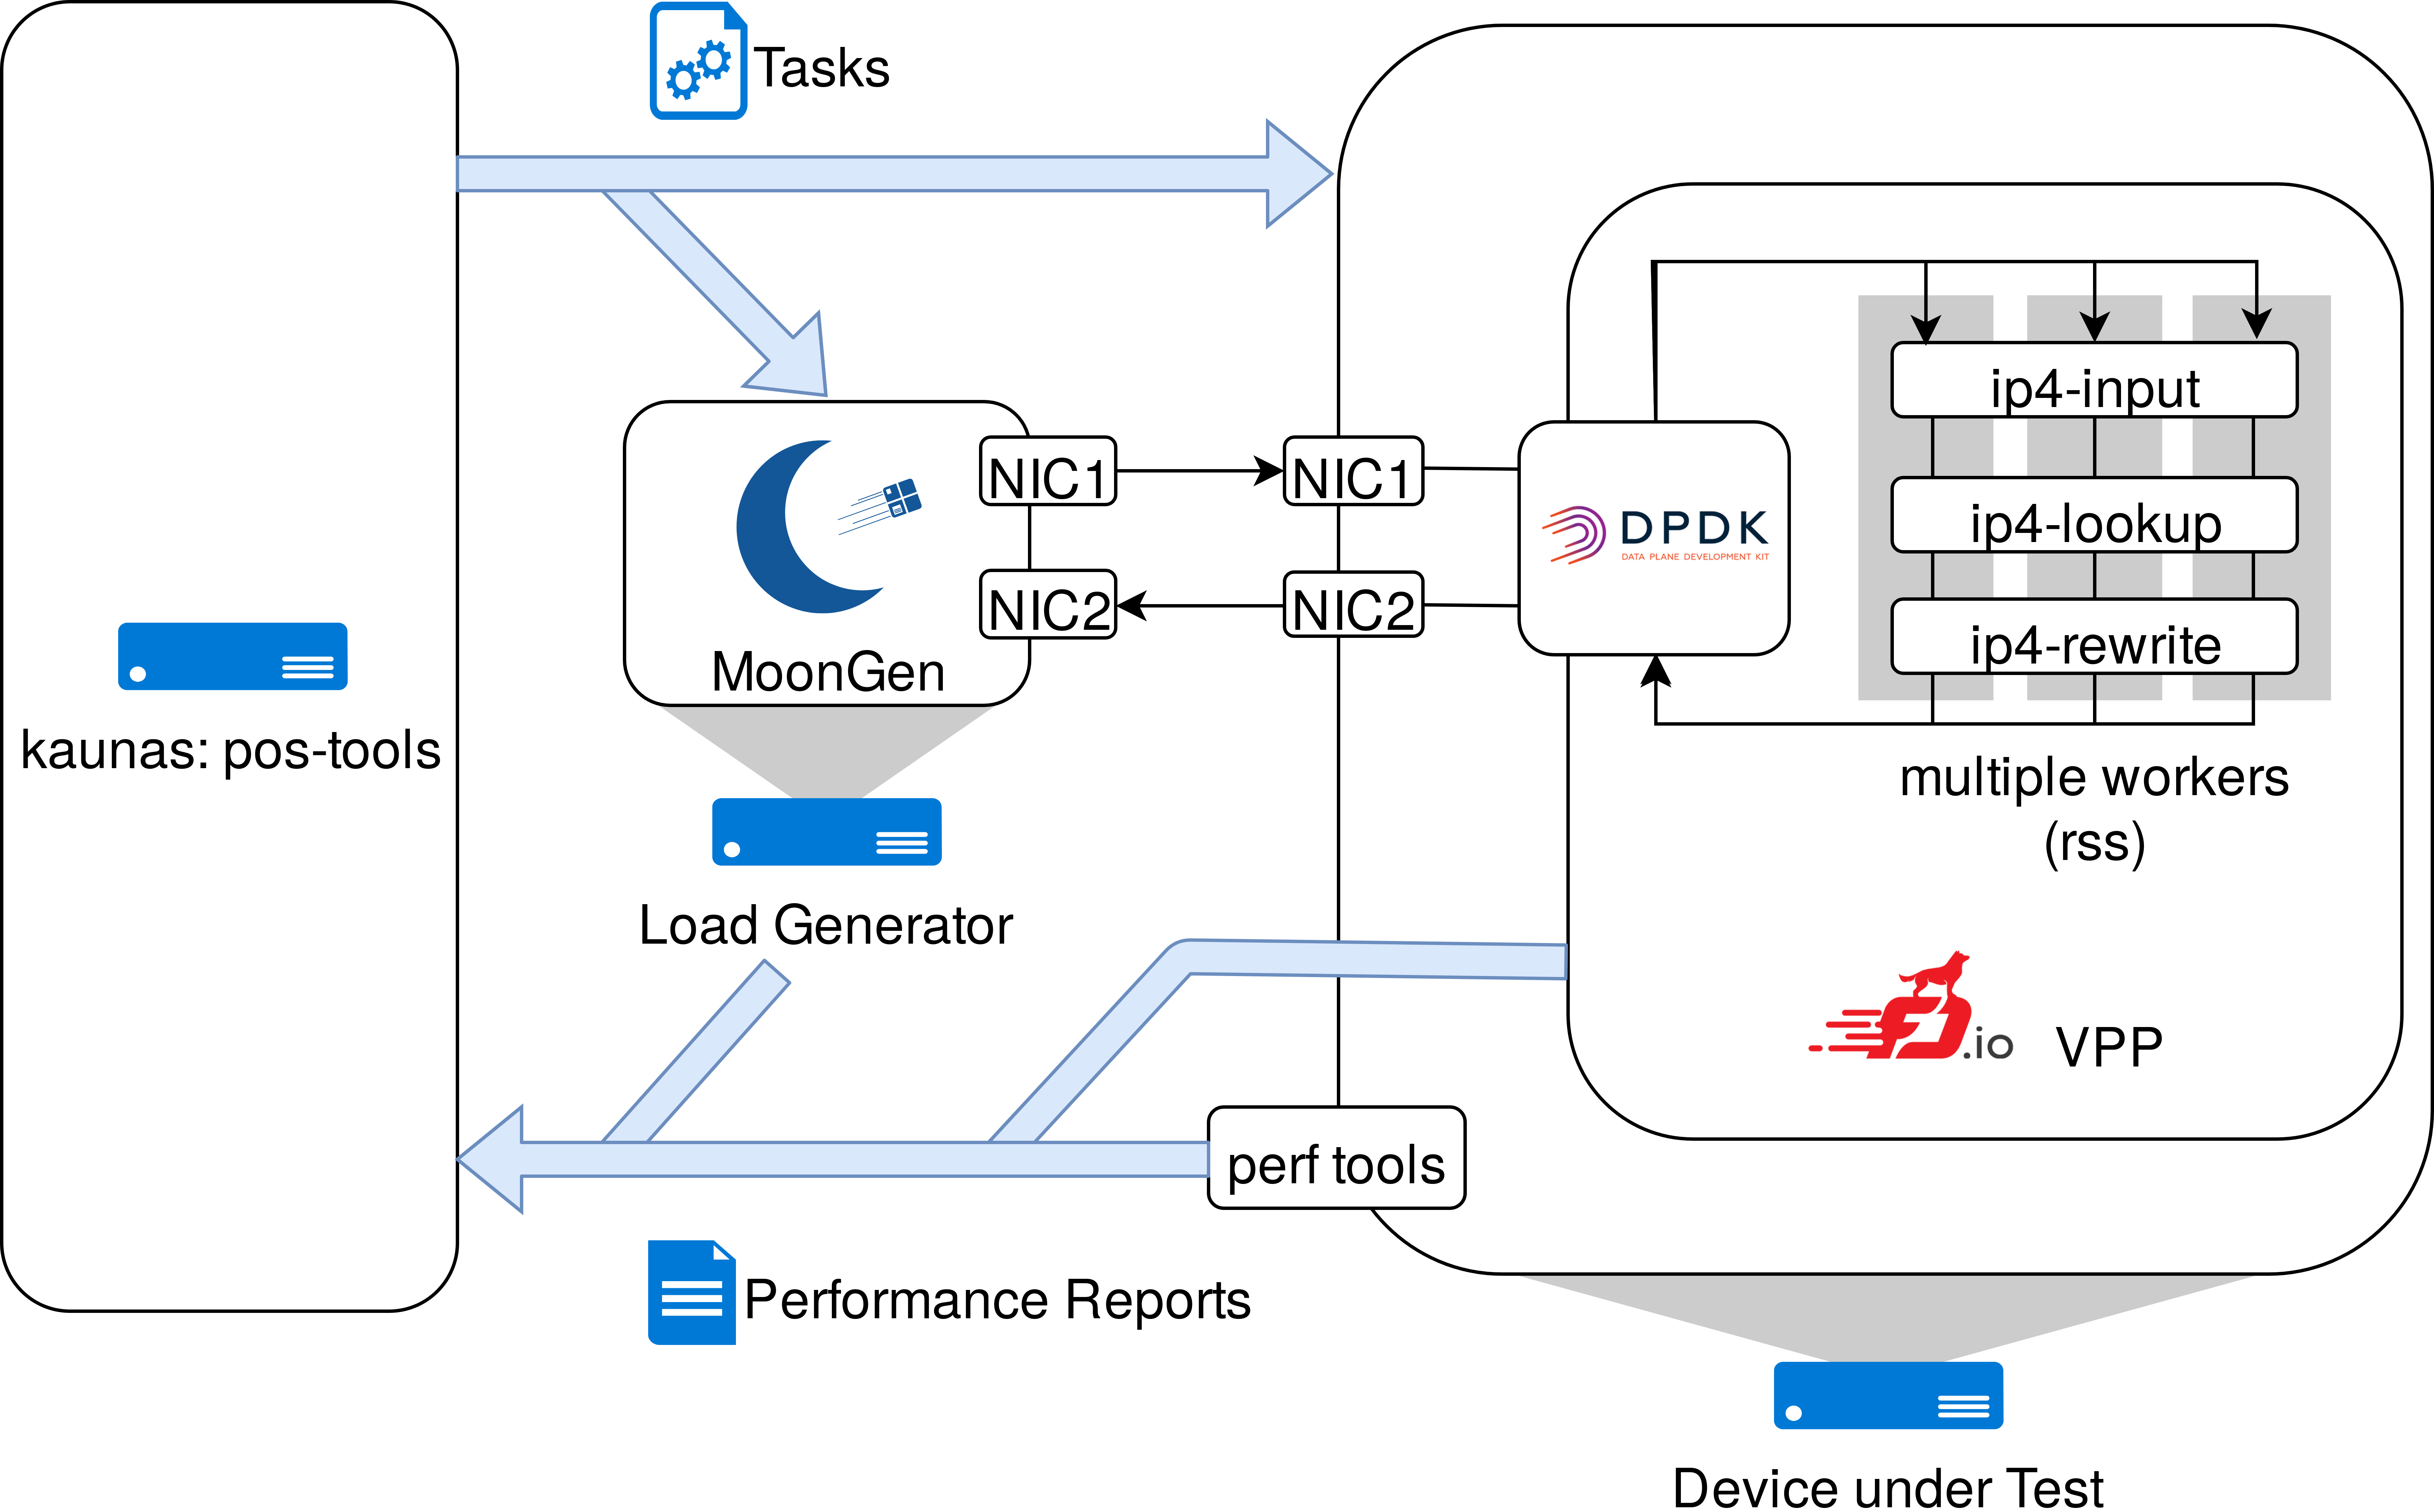
\includegraphics[width=24cm]{pics/topology.png}
		% \includesvg[width=14cm]{../../../pics/topology}
	\end{center}

}

\vfill

\doubletextbox{39ex}{Testing Methodology}{

	\vspace{2ex}
	\footnotesize
	For latency measurements the optimum of throughput to latency has to be found. Otherwise a worst case of latency is triggered, because packet queues fill up. \cite{gallenmuller2015comparison} 

	\vspace{5ex}
	\footnotesize
	VPP properties to test:
	\begin{itemize}
		\item raw forwarding throughput
		\item latency: cache and memory impact
		\item packet processing graphs utilizing multiple cpu cores
		\item testing specific processing nodes / router features
	\end{itemize}

}{Testing Parameters}{

	\vspace{2ex}
	\footnotesize
	MoonGen \cite{moongen-imc2015} scripts can generate testing load according to the following testing parameters:
	\begin{itemize}
		\item packet rate
		\item packet size
		\item traffic type (ethernet, UDP, multiple flows)
		\item traffic pattern (inter packet gaps)
		\item grant warmup time
	\end{itemize}

	\footnotesize
	Gathered testing results:
	\begin{itemize}
		\item latency histogram
		\item throughput
		\item linux perf stats (cache misses...)
		\item linux perf record (cpu-time spent per symbol)
		\item internal vpp state information
	\end{itemize}

}

\vfill

\doubletextbox{28ex}{l2 Throughput}{

	\footnotesize
	VPP on Intel E5-2640 @ 2.0GHz (cesis) with 10G networking

	\vspace{5ex}
	\centering
	\begin{tabular}[]{ l r r r}
		\footnotesize
		VPP config & max Mpps & stable Mpps & Relative \\
		\midrule
		offered load & 14.86 & 14.86 & 100\% \\
		l2 xconnect & 10.4 & 10.1 & 68\% \\
		l2 bridge: no features & 9.35 & 9.2 & 62\% \\
		l2 bridge: mac-age & 8.62 & 8.6 & 58\% \\
		l2 bridge: mac-learn & 8.51 & 8.3 & 56\% \\
		l2 bridge: mac-learn, mac-age & 8.50 & 8.3 & 56\%
	\end{tabular}

}
{l2 Throughput per Flows}{

	\vspace{-2ex}
	\includegraphics[width=.95\linewidth]{../../statistics/throughput_l2_throughmac_trulyRandom}
	% \includesvg[width=14cm]{../../../pics/topology}

}

\vfill 

% This is the literature box.
% There the most relevant papers related to the presented work are listed.
\notitlesingletextbox{13ex}{
	%\nocite{ancs}%

	\vspace{-1ex}  
	\scriptsize
	\begingroup
		\renewcommand{\section}[2]{}%
		\bibliography{lit}
		\bibliographystyle{abbrv}
	\endgroup
}

\vfill

\end{document}